
% Due thursday

\documentclass{article}

\usepackage[utf8]{inputenc}

\usepackage{amsmath, bm}
\usepackage{graphicx}
\usepackage{amssymb}
\usepackage{float}
\usepackage{caption}
\usepackage{subcaption}
\usepackage{hyperref}
\usepackage{tikz}
\usepackage{layout}

\usepackage[margin=1in]{geometry}
\usepackage{listings}
\usepackage{xcolor}
\usepackage{color, colortbl}
\usepackage{textgreek}
\usepackage{mathrsfs}
\usepackage{savetrees}


\setlength{\parskip}{\baselineskip}%
\setlength{\parindent}{0pt}%
\linespread{0.9}


\definecolor{codegreen}{rgb}{0,0.6,0}
\definecolor{codegray}{rgb}{0.5,0.5,0.5}
\definecolor{codepurple}{rgb}{0.58,0,0.82}
\definecolor{backcolour}{rgb}{0.95,0.95,0.92}

\lstdefinestyle{mystyle}{
    backgroundcolor=\color{backcolour},   
    commentstyle=\color{codegreen},
    keywordstyle=\color{magenta},
    numberstyle=\tiny\color{codegray},
    stringstyle=\color{codepurple},
    basicstyle=\ttfamily\footnotesize,
    breakatwhitespace=false,         
    breaklines=true,                 
    captionpos=b,                    
    keepspaces=true,                 
    numbers=left,                    
    numbersep=5pt,                  
    showspaces=false,                
    showstringspaces=false,
    showtabs=false,                  
    tabsize=2
}

\lstset{style=mystyle}



\begin{document}

\title{GA3: Heat Exchanger Performance Report}
\author{lwp26}
\date{May 2024}
\maketitle 

\section{Introduction}

\section{Uncertainty Analysis}

\subsection{Preliminary Analysis}

\begin{equation}
    \dot{Q} = f(L_\text{tube}, \dot{m}_1, \dot{m}_2, T_{1in}, T_{2in}) = f(x_1, x_2, \ldots, x_N)
\end{equation}

The relative uncertainty due to variable $i$ is found numerically by:

\begin{equation}
    u_i(\dot{Q}) \approx \frac{ \left| \dot{Q}(x_i + \delta x_i) - \dot{Q}(x_i) \right|}{\dot{Q}(x_i)}
\end{equation}

An initial test was performed to determine the sensitivity of $\dot{Q}$ to baffle spacing, pitch and length.
The absolute uncertainty in baffle spacing, pitch and length is taken to be 1mm.
This represents a high relative uncertainty in the pitch due to the empirical method used in the software.
The relative uncertainty in calculated $\dot{Q}$ was found to be 0.00546\%, 0.58286\% and 0.11430\% for baffle spacing, pitch and length respectively.
This shows that an uncertainty in baffle spacing has negligible effect and is not considered in further analysis.

% Due to the large number of inputs, a Monte Carlo simulation was used to determine the uncertainty in $\dot{Q}$.

For all 2024 designs the number of tubes and baffles are equal across cross sections.

\subsection{Uncertainty of Inputs}

To perform further uncertainty analysis the uncertainty in input variables must be determined.
For length the uncertainty can be estimated from CAD drawings and manufacturing processes.
The uncertainty in the pitch is harder to determine.

Given that the CAD drawings are available, it makes sense to define a true average pitch and compare this to the calculated pitch to determine the uncertainty.
The true average pitch is defined as the average edge length of a network spanning a given hot section.
For all designs in 2024 the hot sections are circularly symmetric and so the average pitch is the same for all hot sections.

\begin{minipage}[t]{0.29\textwidth}
    \centering
    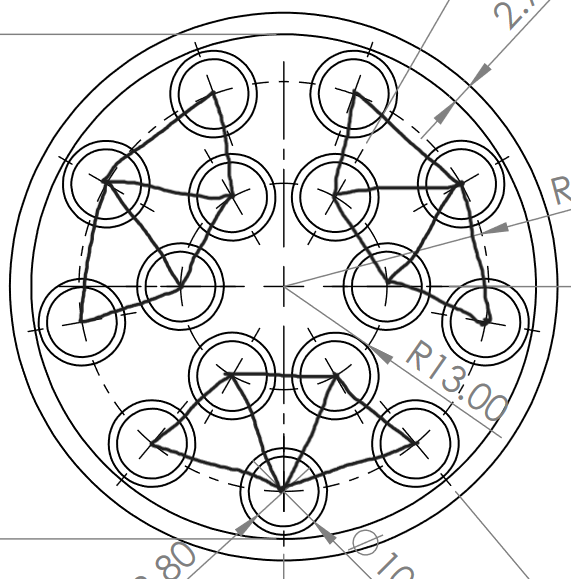
\includegraphics[width=0.8\textwidth]{tube_network.png}
    \captionof{figure}{Three tube networks in our heat exchanger design}
    \label{fig:tube_network}
\end{minipage}
\begin{minipage}[t]{0.69\textwidth}
    \centering
    \begin{tabular}{|c|c|c|}
        \hline
        Design & Calculated Pitch (mm) & True Average Pitch (mm) \\
        \hline
        A & 16.33 & 12.00 \\
        B & 16.33 & 15.41 \\
        C & 16.33 & 14.67 \\
        D & 15.21 & 12.00 \\
        E & 14.49 & 15.13 \\
        \hline
    \end{tabular}
    \captionof{table}{Pitch Comparison}
    \label{tab:pitch_comparison}
\end{minipage}



\begin{figure}[H]
    \centering
    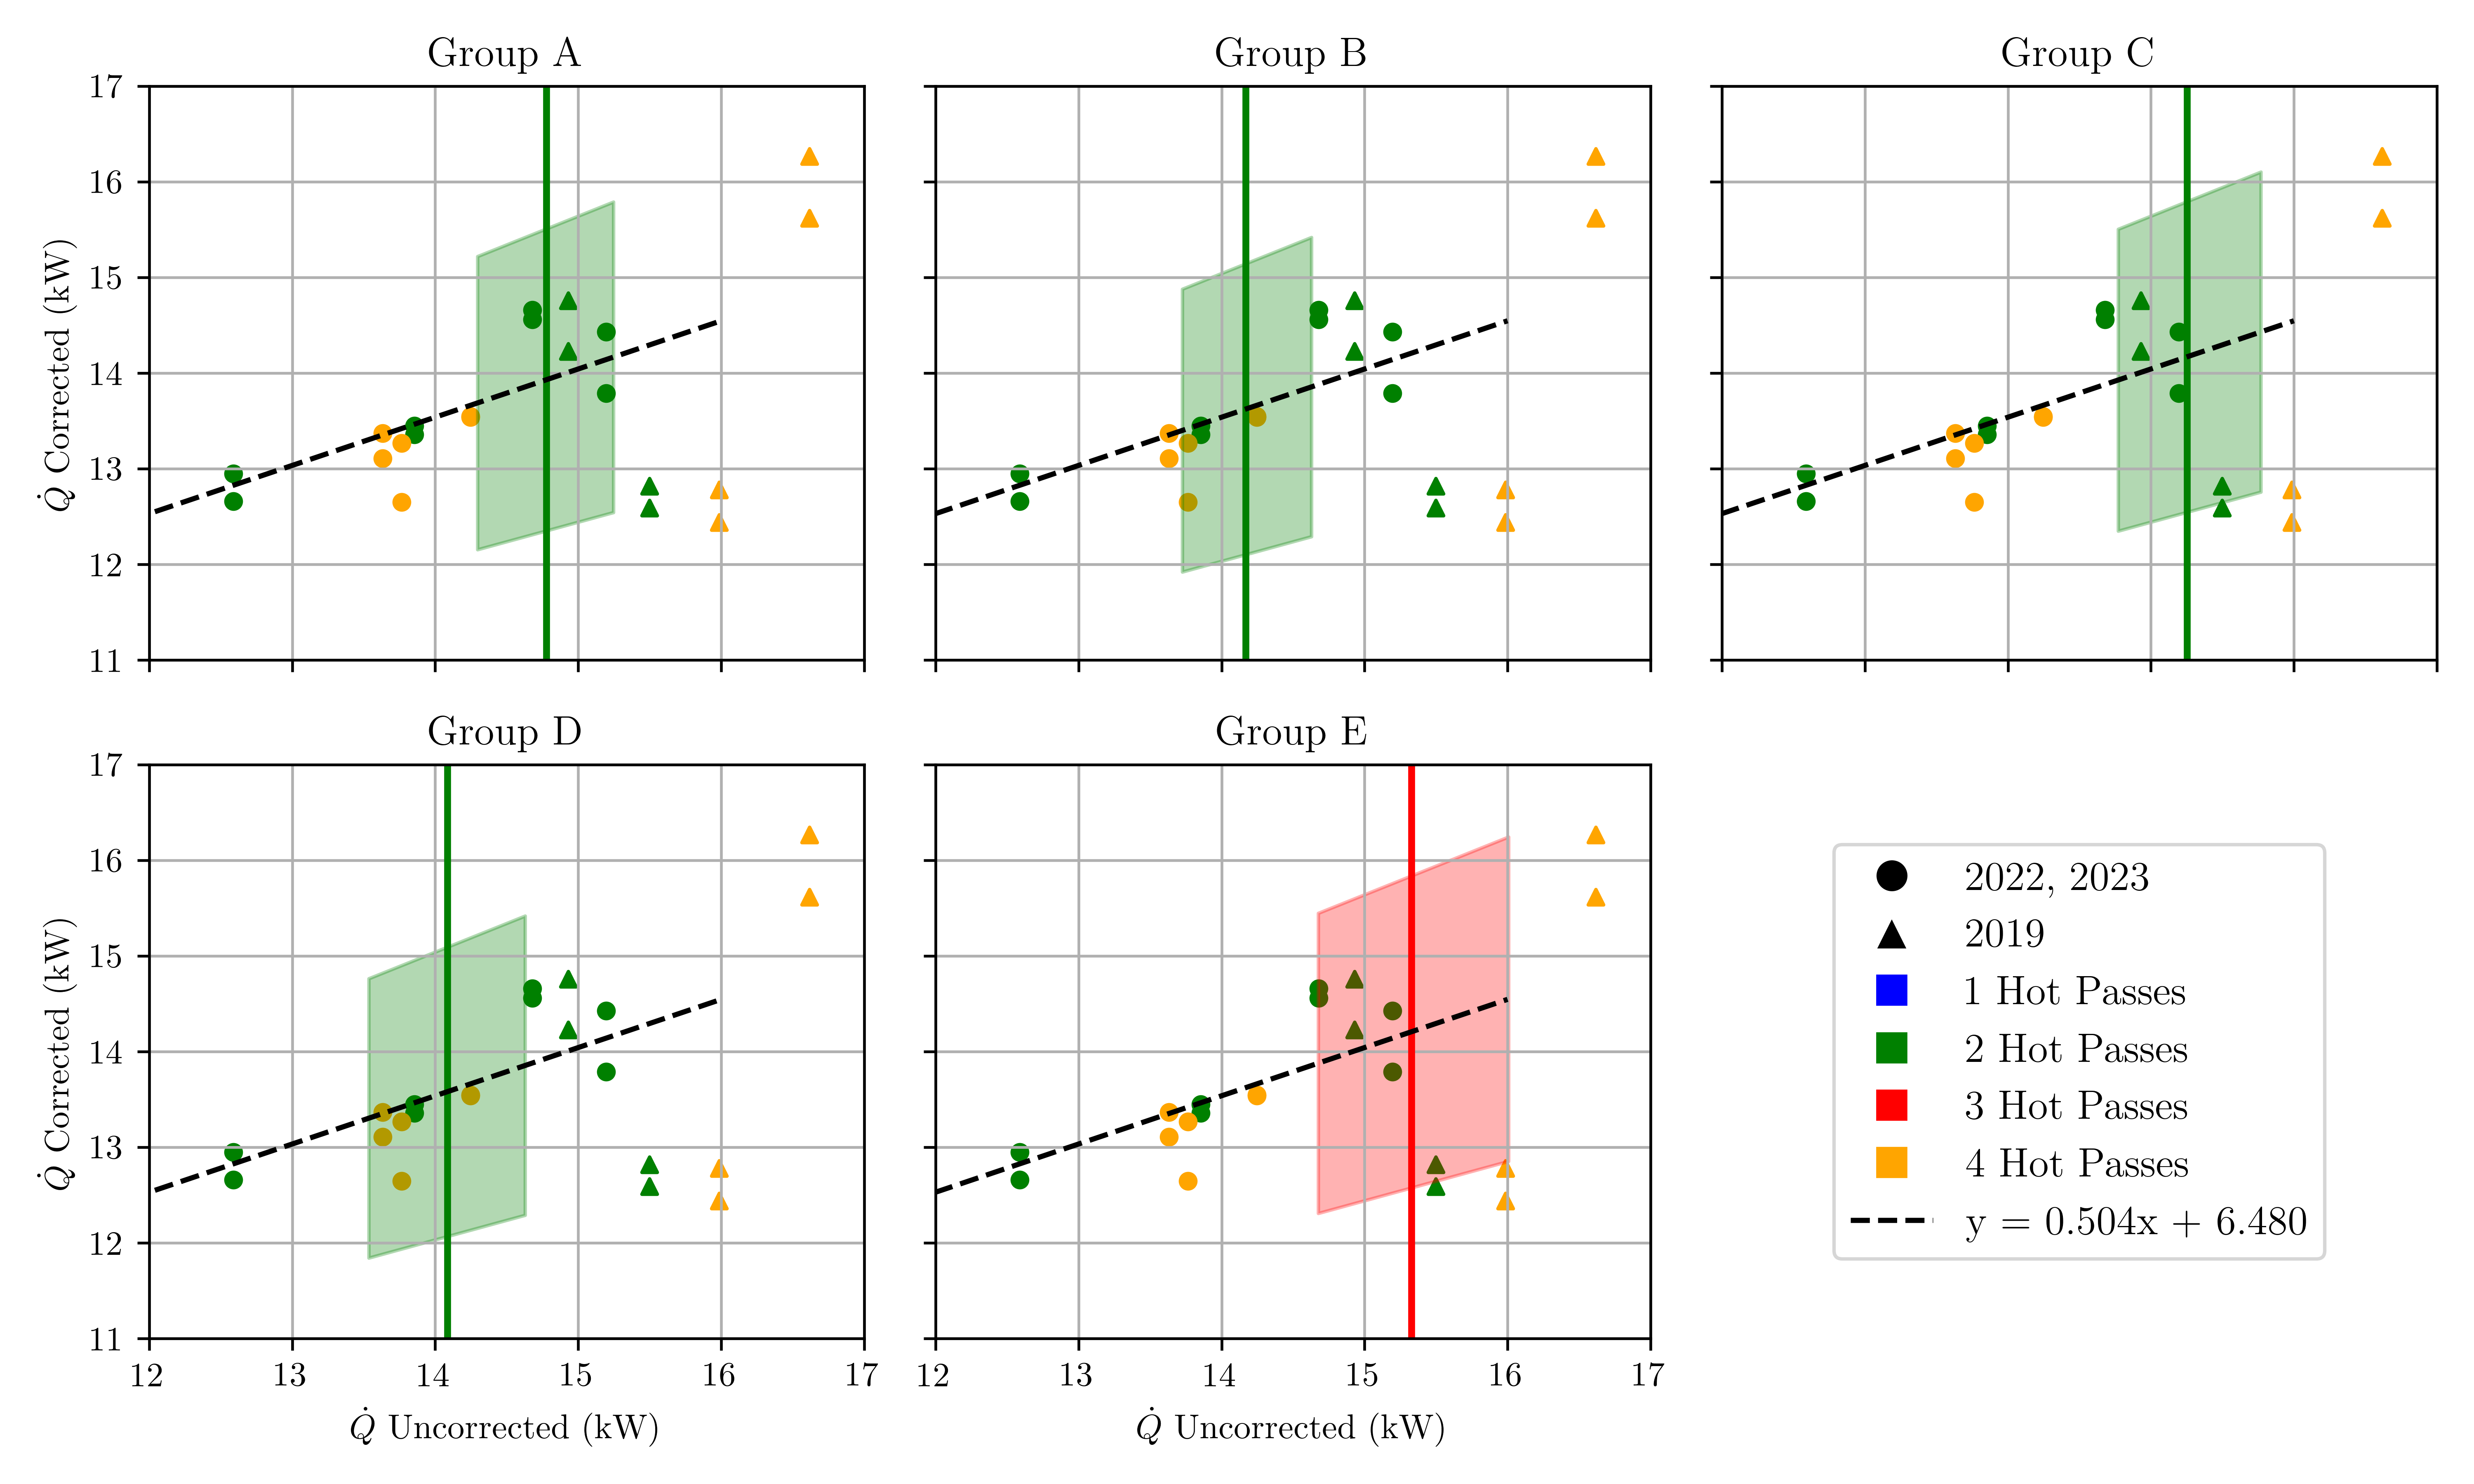
\includegraphics[width=0.99\textwidth]{Qdot_uncertainty_bands.png}
    \caption{$\dot{Q}$ Uncertainty Regions for 2024 Designs}
    \label{fig:uncertainty}
\end{figure}

\section{Performance Degradation}

Fouling is a common issue in heat exchangers, leading to a reduction in heat transfer.
This can be due to a variety of mechanisms depending on the fluid, geometry and operating conditions.

\subsection{Performance Comparison}


\begin{figure}[H]
    \centering
    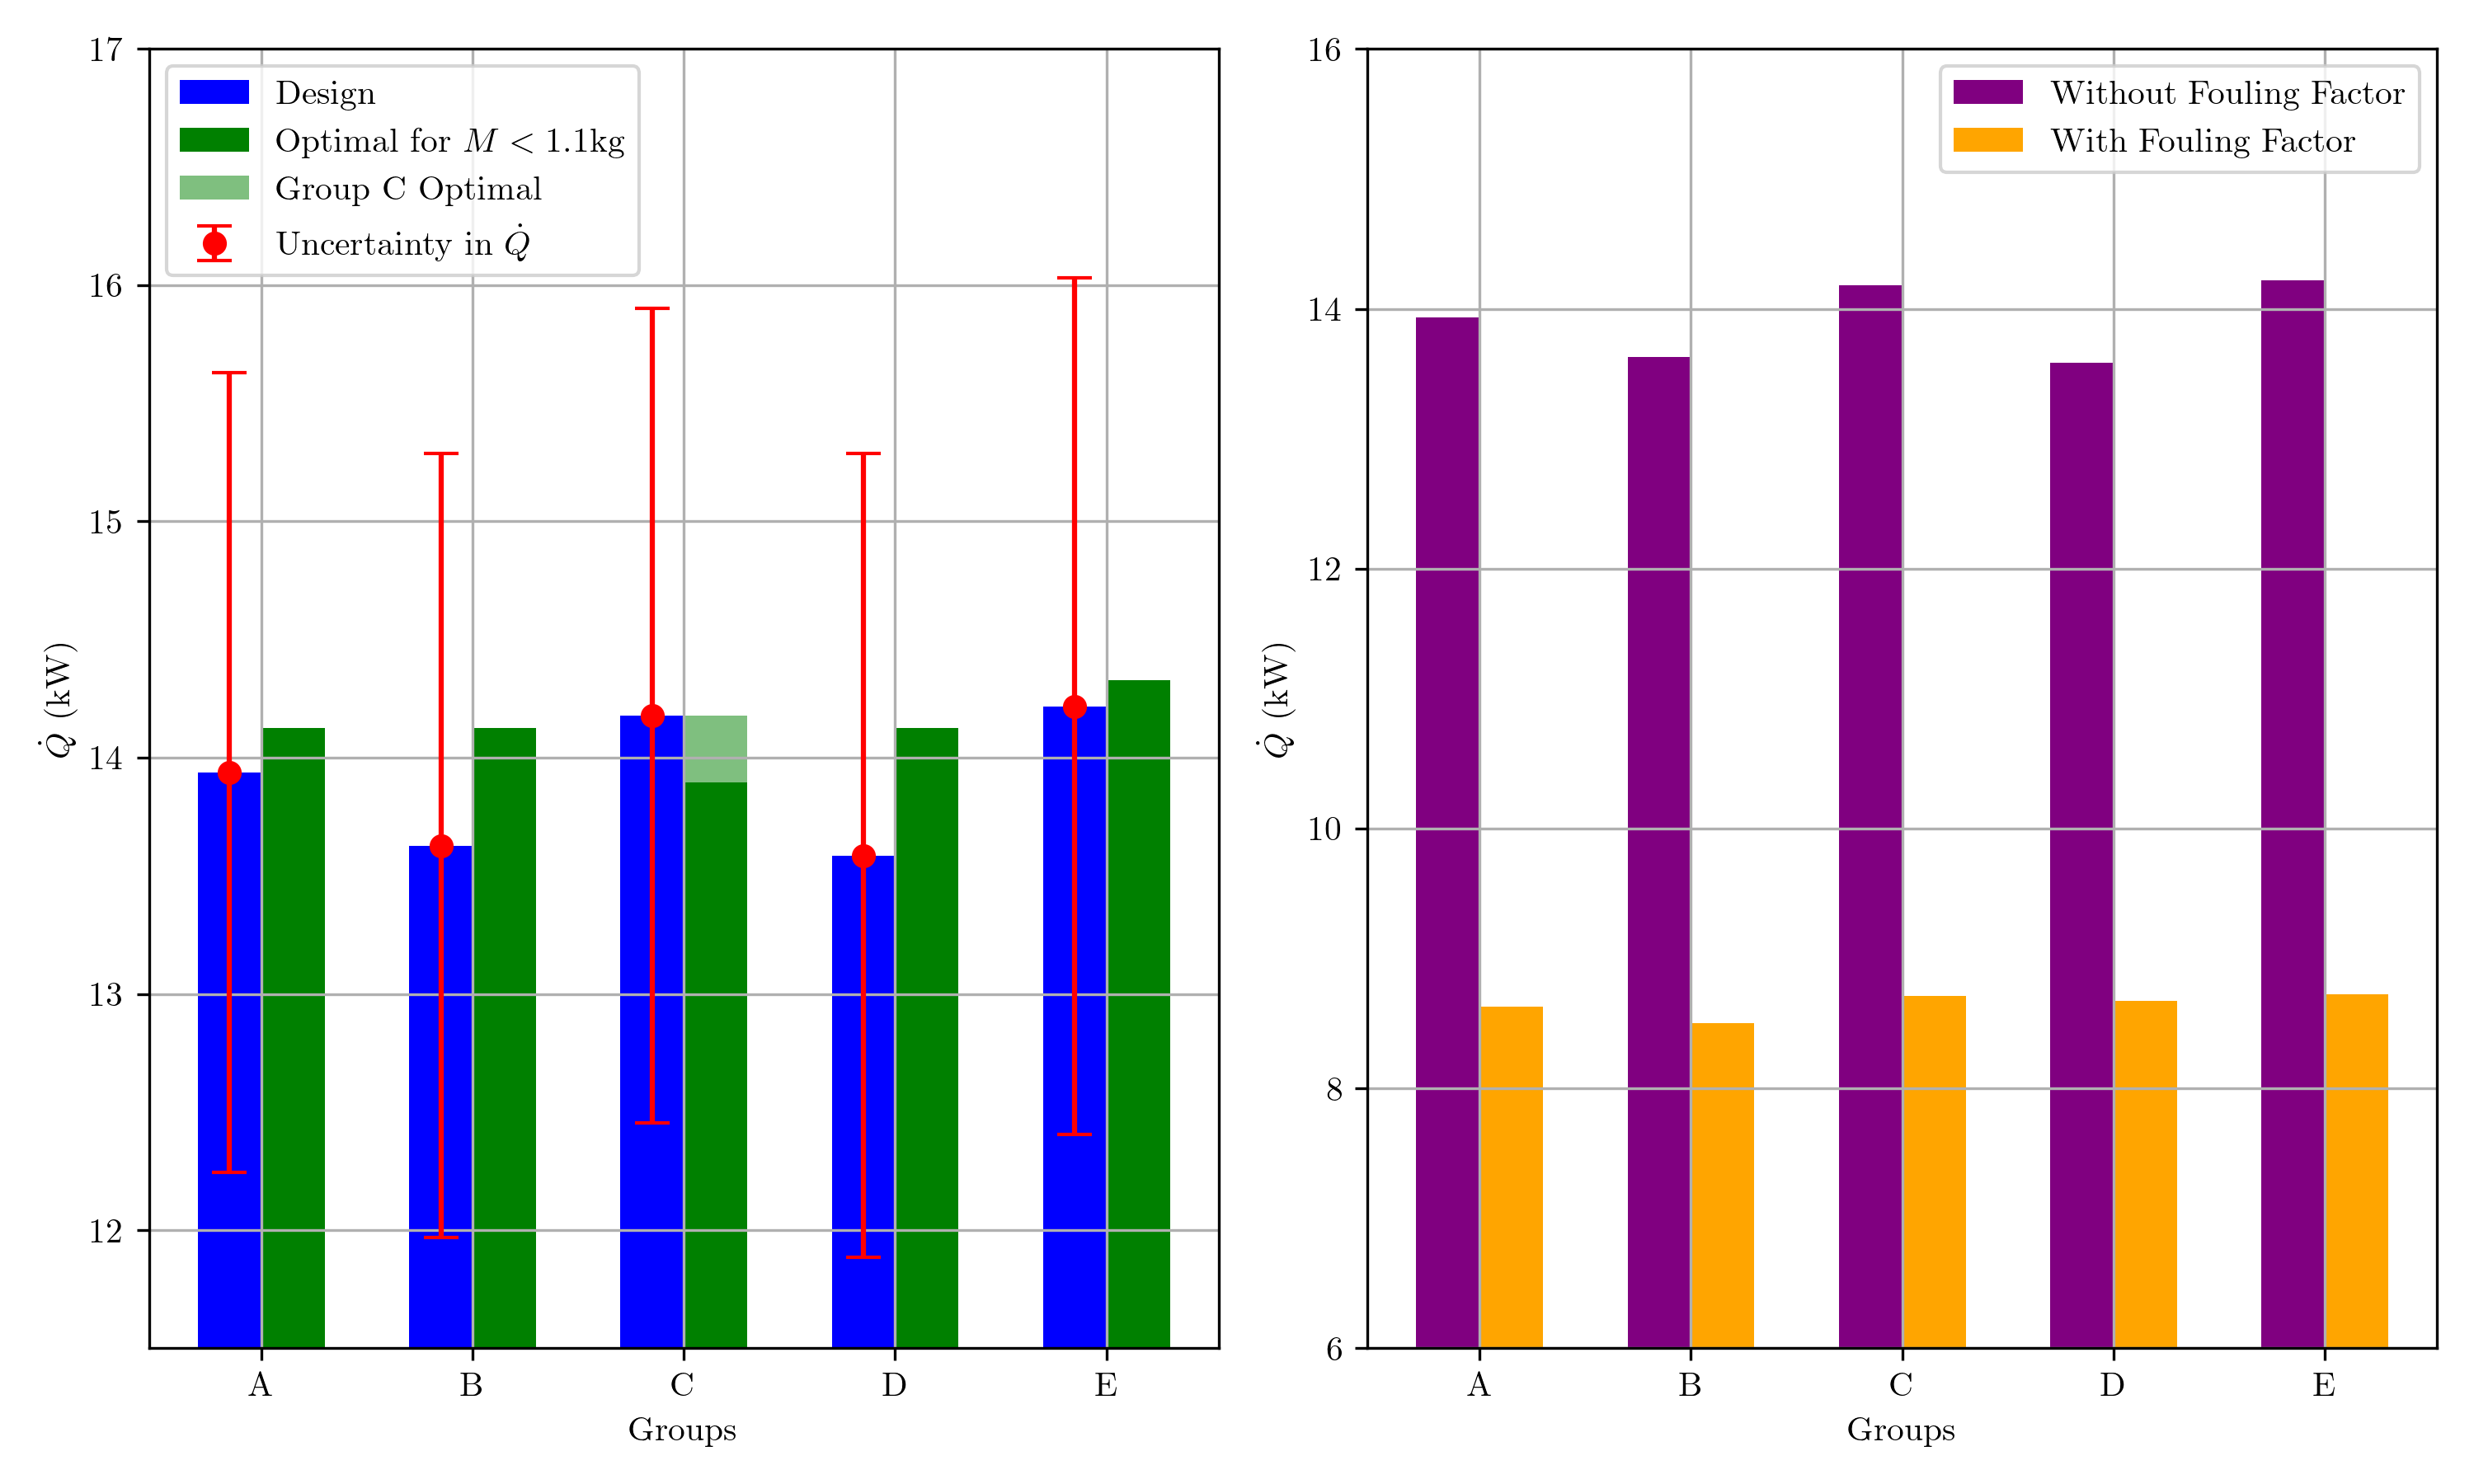
\includegraphics[width=0.8\textwidth]{2024comparison.png}
    \caption{2024 Performance Comparison}
    \label{fig:2024_performance}
\end{figure}

\begin{thebibliography}{9}

    %Endres, SC, Sandrock, C, Focke, WW (2018) “A simplicial homology algorithm for lipschitz optimisation”, Journal of Global Optimization.
    
      \bibitem{handout}
      J. V. Taylor and J. C. Massey
      \emph{GA3 Heat Exchanger Handout}
      University of Cambridge,
      2024.
    
      \bibitem{HeatTransfer}
      Holman J. P.
      \emph{Heat Transfer. 10th ed.}
      McGraw-Hill,
      2010.

      \bibitem{fouling}
      M. Ratel, Y. Kapoor, Z. Anxionnaz-Minvielle, L Seminel, B. Vinet
      \emph{INVESTIGATON OF FOULING RATES IN A HEAT EXCHANGER USING AN INNOVATIVE FOULING RIG}
      International Conference on Heat Exchanger Fouling and Cleaning
      2013

\end{thebibliography}


\end{document}